\documentclass[12pt, oneside]{book}   	% use "amsart" instead of "article" for AMSLaTeX format
\usepackage{geometry}                		% See geometry.pdf to learn the layout options. There are lots.
\geometry{a4paper}                   		% ... or a4paper or a5paper or ... 
%\geometry{landscape}                		% Activate for rotated page geometry
%\usepackage[parfill]{parskip}    		% Activate to begin paragraphs with an empty line rather than an indent
\usepackage{graphicx}				% Use pdf, png, jpg, or eps§ with pdflatex; use eps in DVI mode
								% TeX will automatically convert eps --> pdf in pdflatex		
\usepackage{amssymb}
\usepackage{fancyhdr}
\usepackage{color}
\usepackage[latin1]{inputenc}
\usepackage{amsmath}
%SetFonts

%SetFonts
\pagestyle{fancy}
\begin{document}
\thispagestyle{empty}
\hspace{10cm}
Release date 26-02-2016
\\
\\
\begin{center}
{\huge Software Engineering 2:}
{\huge MyTaxiService}
\end{center}
\vspace*{\fill}
\begin{center}
\textbf{\huge Design Document} 
\\
\large{V2.0}
\end{center}
\vfill
\begin{center}
{\large Dimitar Anastasovski, Marco Colombo}
\end{center}
\clearpage
\pagestyle{plain}
\tableofcontents
\setcounter{page}{1}
\clearpage
\chapter{Introduction}
\section{Purpose}
This document describes the system architecture and design of MyTaxiService system. Each component is described in terms of its external interfaces and the dependencies on other components. It will form the basis of the planning of the development phase and will be updated using the results from the various development iterations to come to complete architectural design.  The architecture review will allow us to identify what are the weaknesses or strengths of the proposed architecture as well as we hope to obtain a list of suggested changes to improve it. It is intended to capture and convey the significant architectural decisions which have been made on the system.
\section{Scope}
This document applies to the overall design of the system. It contains information relating to the architectural design of the software, the Structure of the Database, and of the physical servers hosting the site.
The main accent is to simplify and optimize the access of passengers to the system and to guarantee fair management of taxi queues. We will build flexible and user-friendly web application and a mobile application that will run on Android and IOS mobile phones. This application can be used by anyone who previously will be register on the registration page. After the registration is done the user will have a user name and password that should remember for furthermore usage of the system. The passenger can call a taxi after a successful logging on the application. After that he can call a taxi and he will be informed about the code of the incoming taxi, waiting time. On the other hand taxi drivers will have a mobile application where the major purpose will be to inform the system about their availability, confirmation of a certain call and global map navigation.  City is divided into taxi zones that are uniquely associated with corresponding taxi queues for efficient usage of the system. 
\section{Definitions}
\begin{itemize}
\item \textbf{Request}: Passenger filled form for immediate ride
\item \textbf{Reservation}: Passengers can request for a vehicle at least 2 hours before the ride and can reserve his ride
\item \textbf{User}: Is a customer who already registered and logged into the system
\item \textbf{Taxi driver}: Is a person who legally drives taxi ( with driver license and work license) already registered and logged into the system as a driver
\item \textbf{System}: Is the system that has to be designed
\item \textbf{Taxi zone}: Are the zones in which the city is divided in
\end{itemize}
\section{Abbreviations}
No abbreviations are been used in this document
\section{Acronymous}
\begin{itemize}
\item IEEE Standard 1016-2009 for Information Technology--Systems Design--Software Design Descriptions
\item Specification Document: myTaxiService Project 
\end{itemize}
\section{Document Structure}
This document is divided in four parts with clean and non-ambiguity description of the whole system.
\begin{itemize}
\item Chapter 1: General description and basic information of the system
\item Chapter 2: Architectural design, which introduces the components of the system and describes the way components interact with specific tasks.
\item Chapter 3: Algorithm design, focused on the most interesting part of the system
\item Chapter 4: User interface design, providing an overview on how the user can interact with the system.
\item Chapter 5: Requirements traceability, that explains the requirements defined in the RASD into the design elements.
\end{itemize}
\chapter{Architectural Design}
\section{Overview}
This document describes the system requirements, operating environment, system and subsystem architecture, files and database design, input formats, output layouts, human-machine interfaces, detailed design, processing logic, and external interfaces.
\section{High level components and interactions}
\begin{itemize}
\item Guest Handler is component that will provide interface for unregistered users or guest with an option to create a profile.
\item User Handler is component of the system that will provide interfaces for users (passengers) with options of requesting, reserving taxi, managing profile, reporting driver, checking available taxis around him and canceling a ride.
\item Taxi Driver Handler is component of the system that will provide interfaces for taxi drivers with options of confirming a ride, setting availability, reporting a user and canceling a ride.
\item Admin Manager is component of the system that will provide interfaces for administrators with options of viewing reports and banning a user.
\item Queues manager is component that is consisted of three subcomponents: Request Manager, Reservation Manager and Zone Manager. It provides interfaces for other components with options for requesting a taxi, finding zone, reserving a taxi as well as calculating ETA
\end{itemize}
\begin{figure}[h]
\center 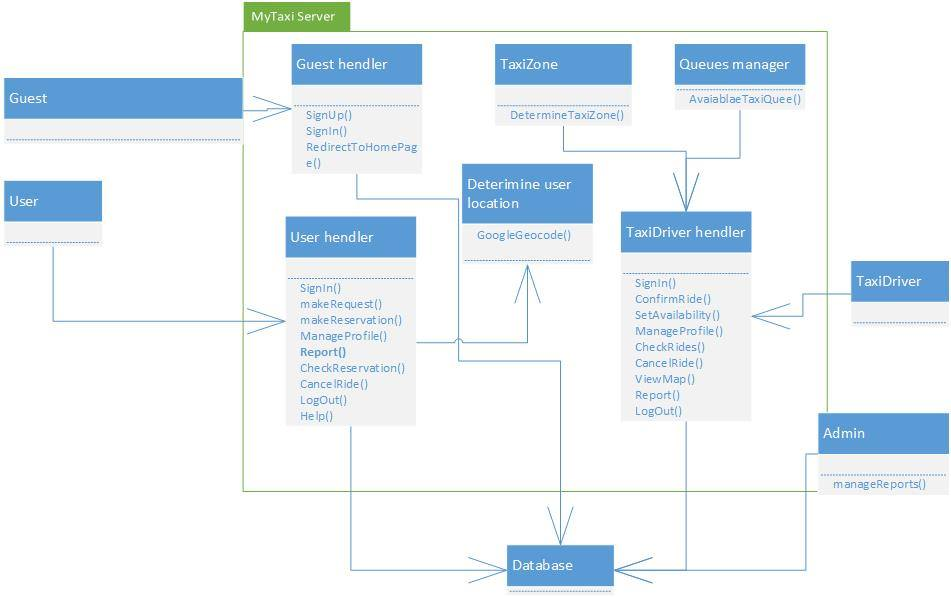
\includegraphics[scale=0.4]{highlevel.jpg}
\end{figure}
\clearpage
\section{Component view}
\begin{figure}[h]
\center 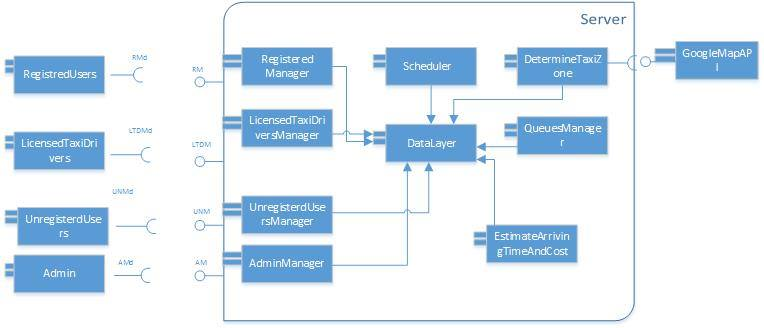
\includegraphics[scale=0.59, angle=90]{component}
\end{figure}
\clearpage
\section{Deployment view}
\vspace{3cm}
\begin{figure}[h]
\center 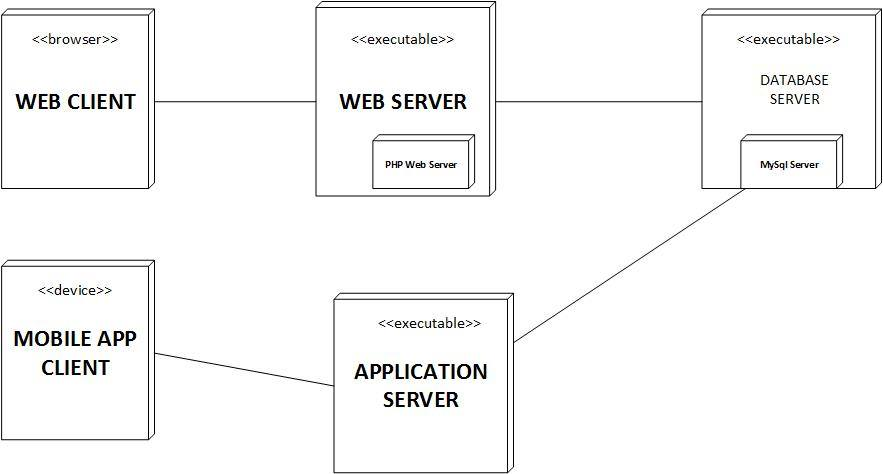
\includegraphics[scale=0.5]{deployment}
\end{figure}
\clearpage
\section{Runtime view}
\vspace{3cm}
\begin{figure}[h]
\center 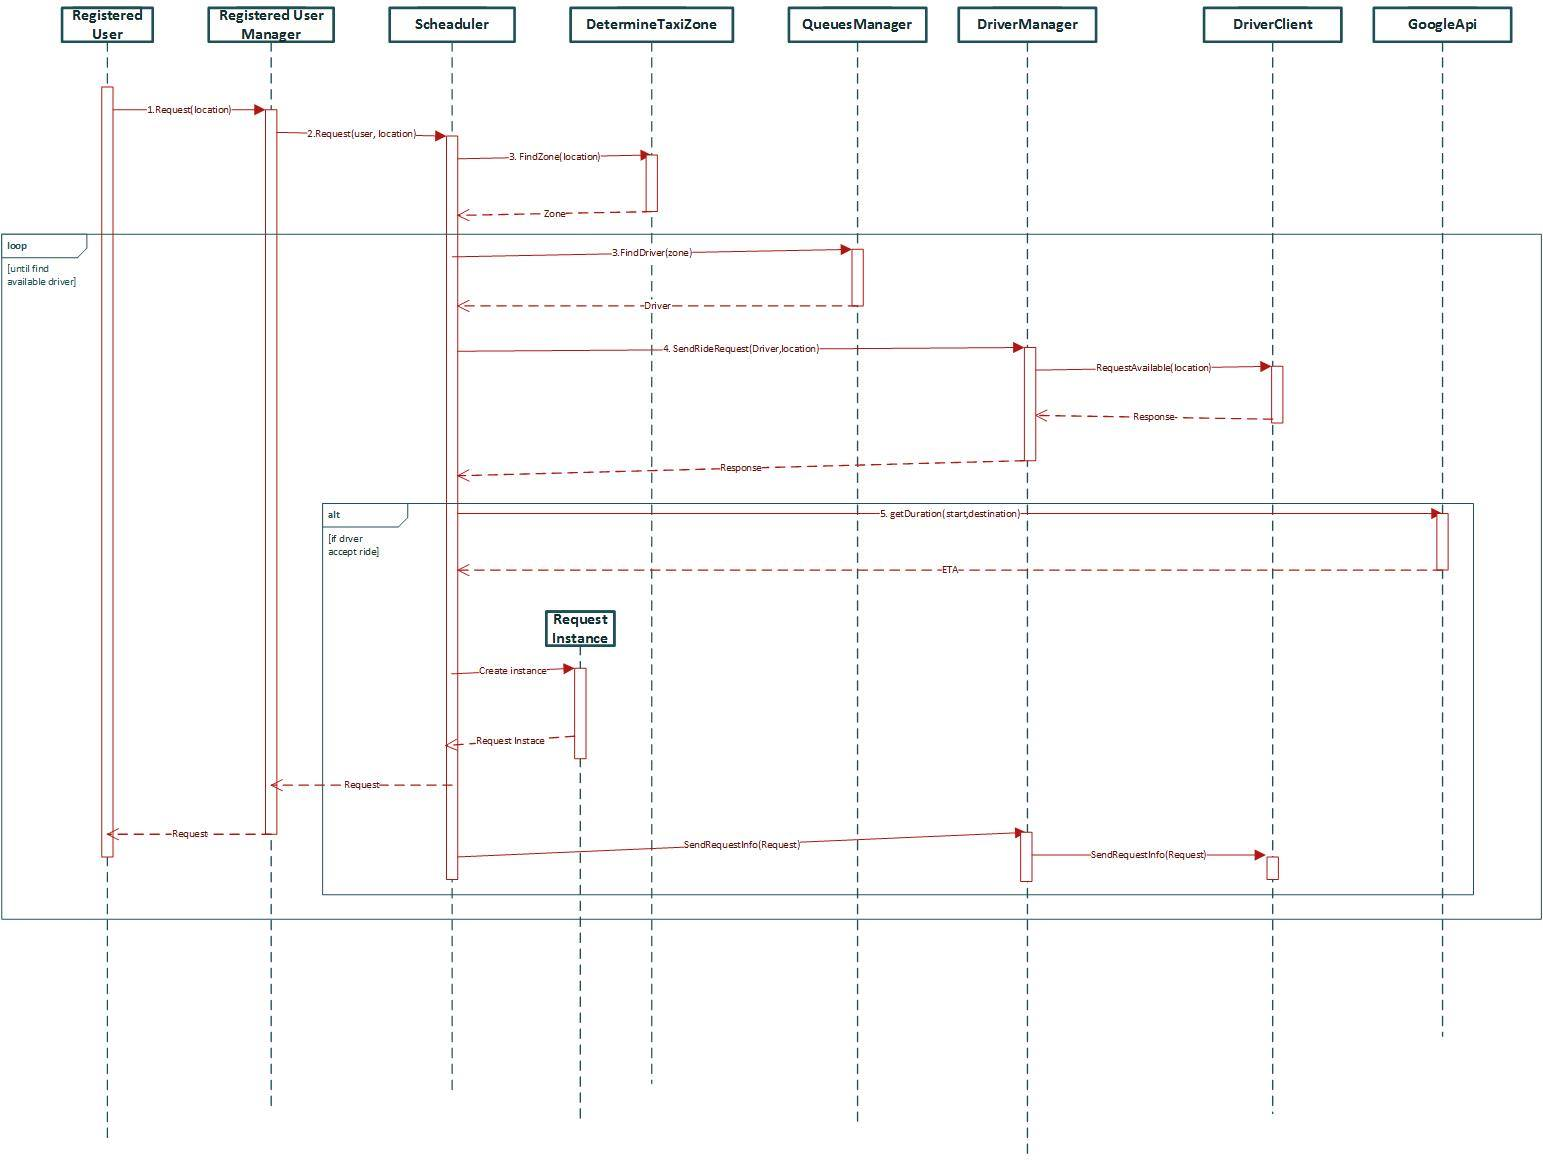
\includegraphics[scale=0.3]{runtime}
\end{figure}
\begin{figure}[h]
\center 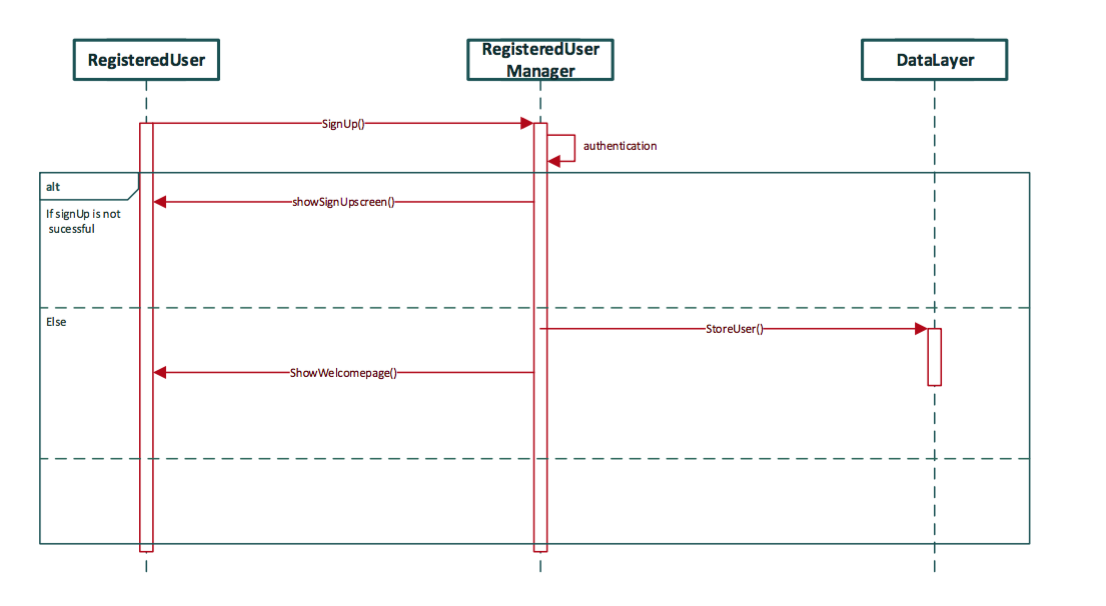
\includegraphics[scale=0.5, angle=90]{runtime3}
\end{figure}
\clearpage
\begin{figure}[h]
\center 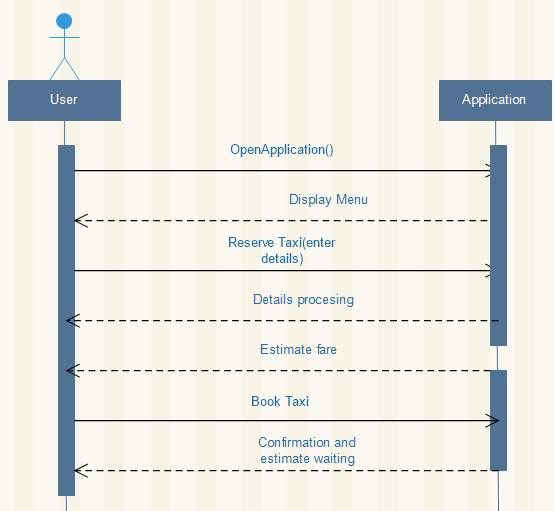
\includegraphics[scale=0.5]{reservetaxi}
\end{figure}
\vspace{3cm}
\begin{figure}[h]
\center 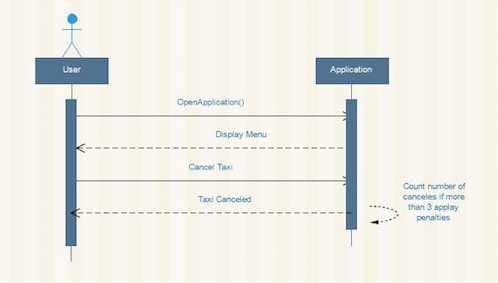
\includegraphics[scale=0.5]{cancelreservation}
\end{figure}
\section{Component interfaces}
\begin{itemize}
\item \textbf{RegisteredUsers: }is a module where clients who already sign up can access their account and can use the features of the application. This component contains sign in module for authentication the users and its communicating with \textbf{RegisteredManager}.
\item \textbf{LicensedTaxiDrivers: }is a module where licensed taxi drivers access their account and can use the features of the application. This component contains sign in module for authentication the users and its communicating with \textbf{LicensedTaxiDriversManager}.
\item \textbf{UnregisteredUsers: }is a module where guest who don't have an account can sign up for using the features of the application. If the guest click on the sign up button it will be redirected to the sign up form for entering basic information. 
\item \textbf{RegisteredManager: } this module is connected with registered users who already sign up and have their own account. It managing all registered users showing them the home page, notifying the users and etc. and is communicating with \textbf{DataLayer} for storing, deleting or retrieval information that is needed.  
\item \textbf{LicensedTaxiDriversManager: }is managing licensed taxi drivers who are already sign up and have their own account. It is communicating with the taxi drivers notifying them about taxi requests, reservations and their cancelation. It can send and receive notification from the taxi drivers, update information about their availability and accept or declined requests. Also it?s communicating with \textbf{DataLayer} for storing, deleting or retrieval information that is needed. 
\item \textbf{UnregisteredUsersManager: }this module is managing the whole registration process for the guests who don't have an account. It is communicating with DataLayer for notifying the system for a new profile and to store the data in the database system. 
\item \textbf{DataLayer }module is managing the whole data of the system. This module is encrypted and can create, delete, modify, store and update informations when it is required.
\item \textbf{Scheduler }module is managing the informations that is needed for the taxi drivers and users. 
\item \textbf{DetermineTaxiZone }module is determine the zone for the taxies so when the user request taxi 
this module is response for calling the taxi nearest to the customer. Also is taking care to have availably taxis in every zone.
\item \textbf{QueuesManager: }this module is providing functions to manage all the taxis queues of the city. It communicate with \textbf{LicensedTaxiDriversManager} in order to retrieve information about taxi?s availability and eventually move it to the end of the queue.
\item \textbf{EstimateArrivingTimeAndCost: }this module is estimating the arrival time and the cost after a user successful book a taxi. 
\end{itemize}
\clearpage
\section{Selected architectural styles and patterns}
\begin{figure}[h]
\center 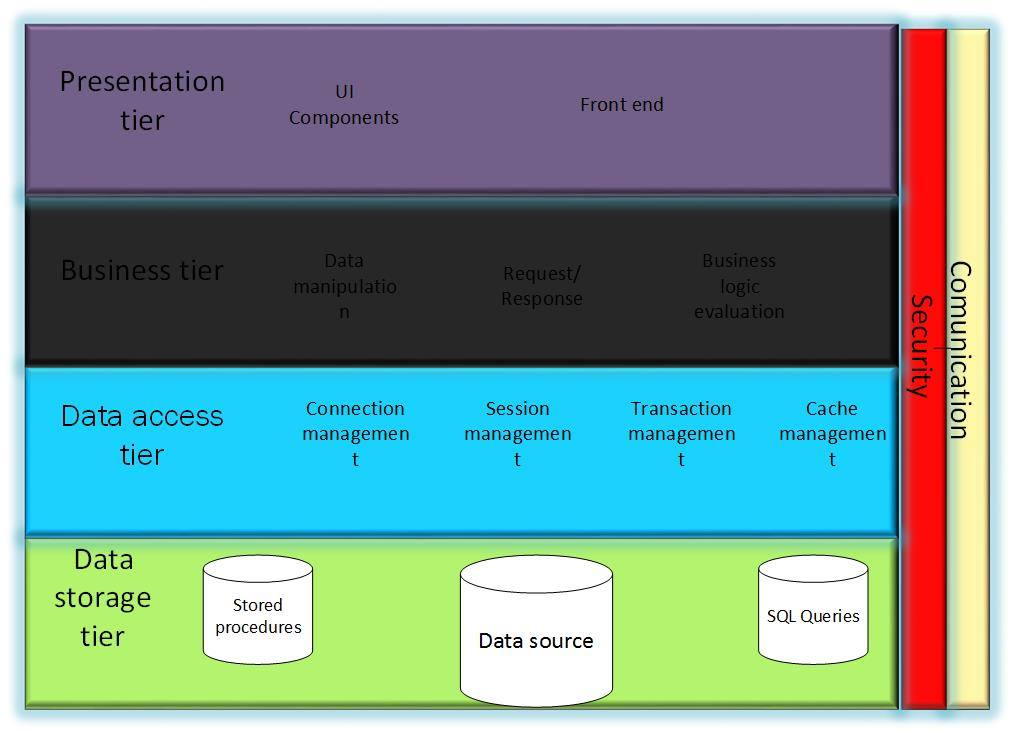
\includegraphics[scale=0.4]{componentinterface}
\end{figure}
\begin{itemize}
\item \textbf{N-Tier} data applications are data applications that are separated into multiple tiers. Also called "distributed applications" and "multitier applications," 
n-tier applications separate processing into discrete tiers that are distributed between the client and the server.A typical n-tier application includes a presentation tier, a middle tier, and a data tier
In addition to the advantages of distributing programming and data throughout a network, n-tier applications have the advantages that any one tier can run on an appropriate processor or operating system platform and can be updated independently of the other tiers.

\item \textbf{Database (Data) Tier} - At this tier, the database resides along with its query processing languages. We also have the relations that define the data and their constraints at this level.

\item \textbf{Application (Middle) Tier} - At this tier reside the application server and the programs that access the database. For a user, this application tier presents an abstracted view of the database. End-users are unaware of any existence of the database beyond the application. At the other end, the database tier is not aware of any other user beyond the application tier. Hence, the application layer sits in the middle and acts as a mediator between the end-user and the database.

\item \textbf{User (Presentation) Tier} - End-users operate on this tier and they know nothing about any existence of the database beyond this layer. At this layer, multiple views of the database can be provided by the application. All views are generated by applications that reside in the application tier.

\item \textbf{Multiple-Tier} database architecture is highly modifiable, as almost all its components are independent and can be changed independently.
\end{itemize}
\begin{figure}[h]
\center 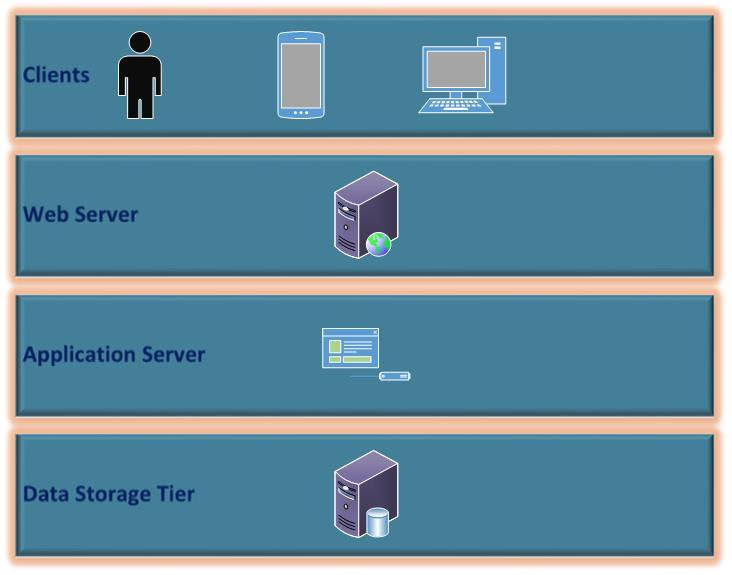
\includegraphics[scale=0.4]{archstyle}
\end{figure}
\clearpage
The model-view-controller pattern proposes three main components or objects to be used in software development:
\vspace{2cm}
\begin{figure}[h]
\center 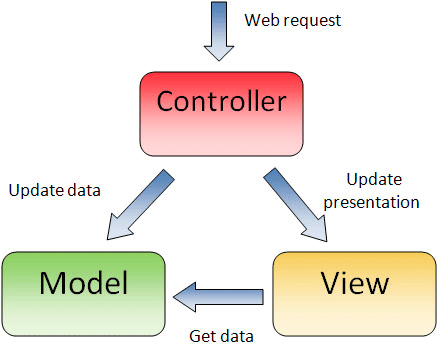
\includegraphics[scale=0.4]{mvc.png}
\end{figure}
\vspace{2cm}
\begin{description}
\item[]- \textbf{Model}, which represents the underlying, logical structure of data in a software application and the high-level class associated with it. This object model does not contain any information about the user interface.
\item[]- \textbf{View}, which is a collection of classes representing the elements in the user interface (all of the things the user can see and respond to on the screen, such as buttons, display boxes, and so forth)
\item[]- \textbf{Controller}, which represents the classes connecting the model and the view, and is used to communicate between classes in the model and view.
\end{description}
When the MVC and three-tier approaches are brought together the View and Controller are considered the presentation tier, the Model exists in the business tier (and has access to many business and data tier modules). To a certain extent the Model could span both the business and data tiers. Writes take considerably more data storage resources than do reads, so separating these into different physical data stores can have huge benefit. It should also identify that the modules for the business and data logic can be numerous. And these exist for maintainability and scalability purposes. It is also reasonable that the Model may access the Data Tier directly without going through a Business Tier module.
\clearpage
\chapter{Algorithm Design}
\begin{figure}[h]
\center 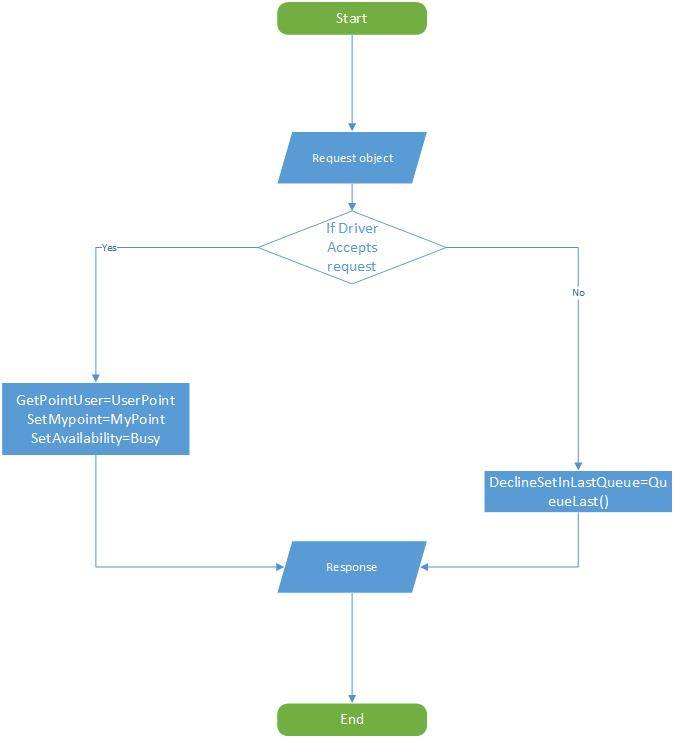
\includegraphics[scale=0.4]{request}
\end{figure}
\clearpage
\begin{figure}[h]
\center 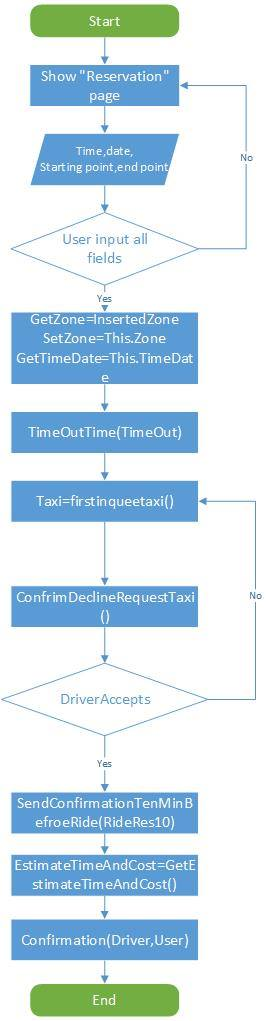
\includegraphics[scale=0.5]{algoreserve2}
\end{figure}
\chapter{User Interface}
\section{User interface design}
\vspace{2cm}
\hspace*{\fill}
\textbf{\large Homepage \& registration page}
\hspace*{\fill}
\begin{figure}[h]
\centering
\includegraphics[scale=0.45]{Homepage.png}
\end{figure}
\\
The passenger can access to the registration page and register himself to the application.
\clearpage
\hspace*{\fill}
\textbf{\large Login}
\hspace*{\fill}
\begin{figure}[h]
\centering
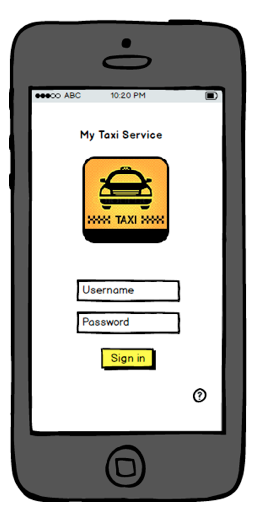
\includegraphics[scale=0.7]{login.png}
\end{figure}
\\
This is the login page. Here the user after entered his data can sign in the application.
\vspace{1cm}
\clearpage
\hspace*{\fill}
\textbf{\large Menu}
\hspace*{\fill}
\\
\begin{figure}[h]
\centering 
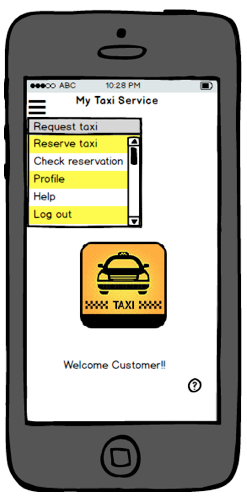
\includegraphics[scale=0.7]{menu.png}
\end{figure}
\\
This is the menu page, here the user can navigate and choose what to do. There are several options like: reserve taxi, check reservation, profile, help or log out.
\clearpage
\hspace*{\fill}
\textbf{\large Reservation}
\hspace*{\fill}
\\
\begin{figure}[h]
\center 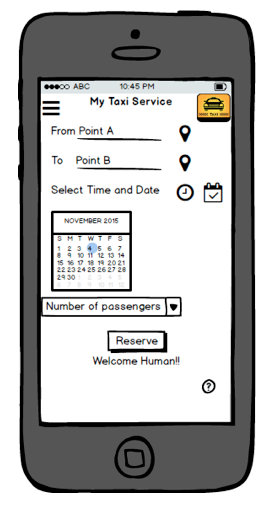
\includegraphics[scale=0.7]{reservation.png}
\end{figure}
\\
Here the passenger can reserve a taxi. He needs to insert the starting and destination point, the date and the number of passenger.
\clearpage
\hspace*{\fill}
\textbf{\large Confirm reservation}
\hspace*{\fill}
\\
\begin{figure}[h]
\center 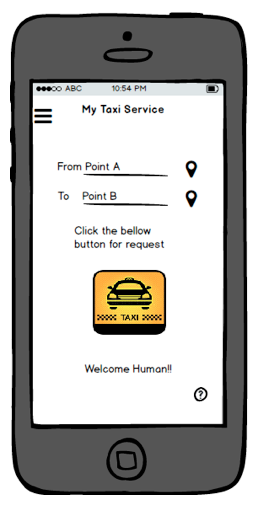
\includegraphics[scale=0.7]{confirmreservation.png}
\end{figure}
\\
In this page the passenger can show a recap of his trip and confirm the reservation by clicking on the button
\clearpage
\hspace*{\fill}
\textbf{\large Recap reservation}
\hspace*{\fill}
\begin{figure}[h]
\center 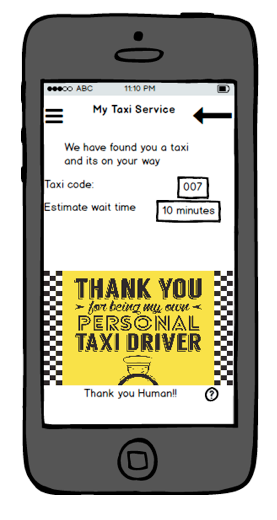
\includegraphics[scale=0.7]{recapreservation.png}
\end{figure}
\\
Here the passenger can see the estimate waiting time and the code of the taxi that will pick him up.
\clearpage
\hspace*{\fill}
\textbf{\large Taxi driver homepage}
\hspace*{\fill}
\\
\begin{figure}[h]
\center 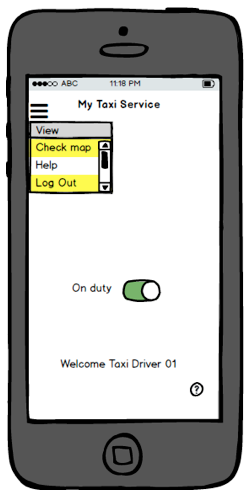
\includegraphics[scale=0.7]{taxidriverhome}
\end{figure}
\\
This is the home page for the taxi driver. He can choose from different option such as: Check map, Help or Log out. Also he can change his status in busy or free.
\clearpage
\hspace*{\fill}
\textbf{\large Taxi driver request}
\hspace*{\fill}
\\
\begin{figure}[h]
\center 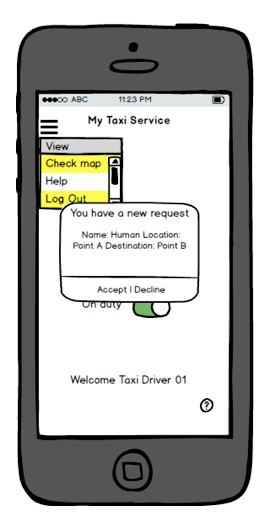
\includegraphics[scale=0.7]{taxirequest}
\end{figure}
\\
This is the notification that the taxi driver will receive when there is a request of a taxi. He can choose if accept or decline this request.
\clearpage
\hspace*{\fill}
\textbf{\large Reservation list for taxi driver}
\hspace*{\fill}
\\
\begin{figure}[h]
\center 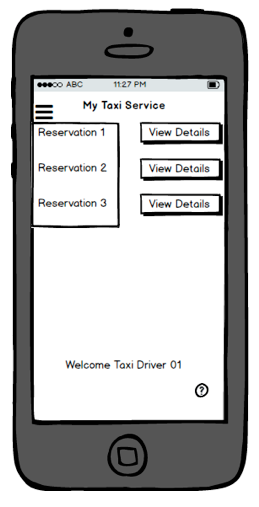
\includegraphics[scale=0.7]{reservationlist}
\end{figure}
\\
Here the taxi driver can give a look at the reservation he has in list and its details.
\clearpage
\hspace*{\fill}
\textbf{\large Taxi driver map}
\hspace*{\fill}
\\
\\
\begin{figure}[h]
\center 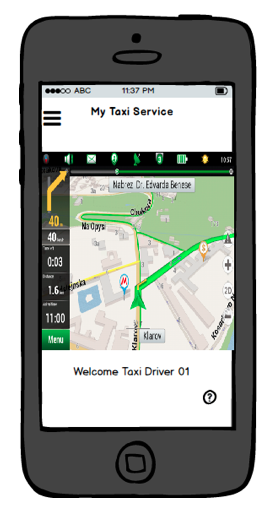
\includegraphics[scale=0.7]{taxidrivermap}
\end{figure}
\\
In this page the taxi driver can see the map of the itinerary for the reservation he chooses.
\clearpage
\chapter{Requirements traceability}
\section{From requirements to diagrams}
\begin{enumerate}
\item \textbf{Allow the registration in the application to the taxi drivers and passengers:}
\begin{itemize}
\item The system should be able to provide a sign up functionality in order to create a new  taxi driver or passenger profiles.
\end{itemize}
\vspace{2cm}
\begin{figure}[h]
\center 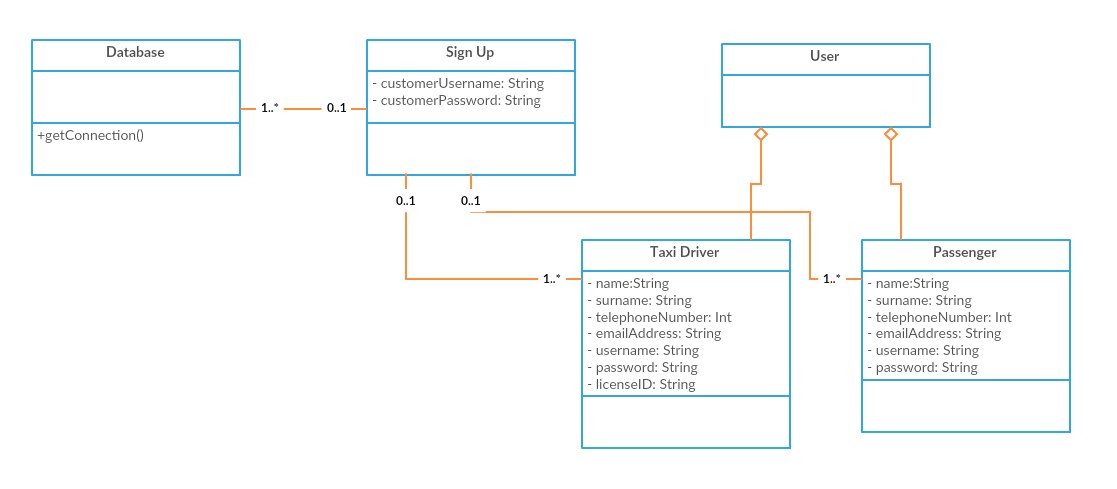
\includegraphics[scale=0.4]{req1}
\end{figure}
\clearpage
\item \textbf{Simplify the access of passengers to the taxy service:}
\begin{itemize}
\item The system has to provide the possibility to the passenger to reserve a taxi
\item The system has to provide both a web application and mobile application in order to allow the passenger to save his time.
\end{itemize}
\vspace{2cm}
\begin{figure}[h]
\center 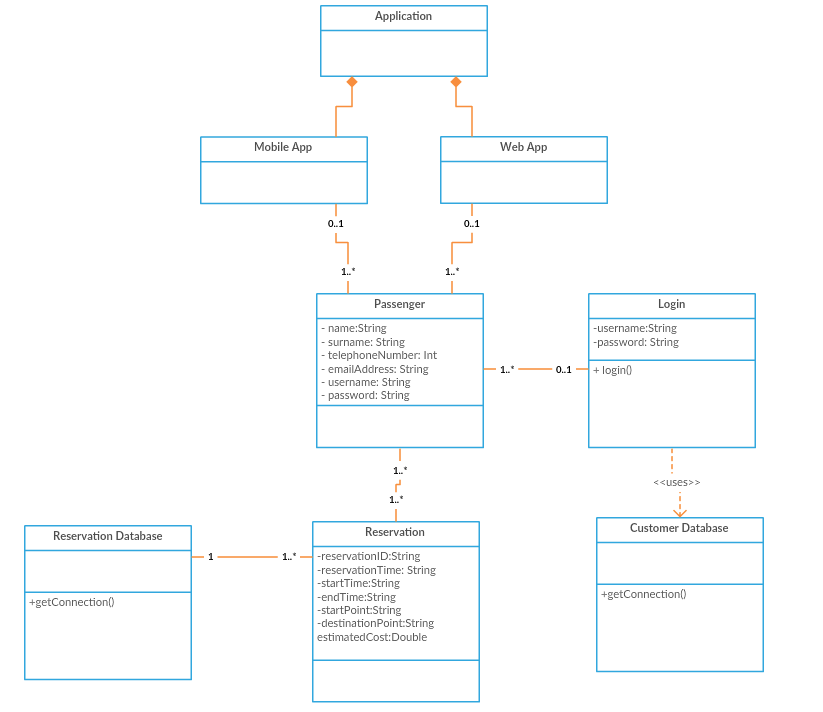
\includegraphics[scale=0.5]{req2}
\end{figure}
\clearpage
\item \textbf{Allow passenger to view if there is any taxi driver free:}
\begin{itemize}
\item The system has to provide a functionality that allow a passenger to view if there is any free taxi driver for the desired route.
\end{itemize}
\vspace{2cm}
\begin{figure}[h]
\center 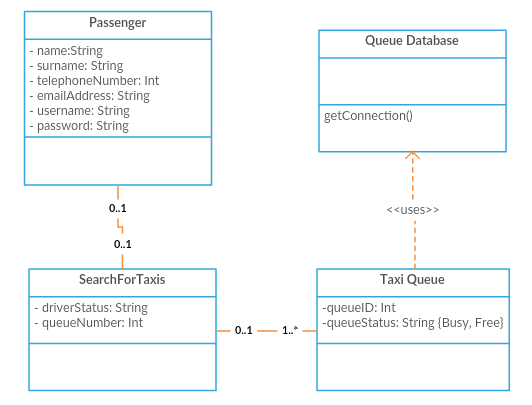
\includegraphics[scale=0.7]{req3}
\end{figure}
\clearpage
\item \textbf{Divide the city into different areas covered by some taxi drivers, organized in queues:}
\begin{itemize}
\item The system has to provide a functionality to divide the city in some areas
\item The system has to organize the taxi of these areas into queues
\end{itemize}
\vspace{2cm}
\begin{figure}[h]
\center 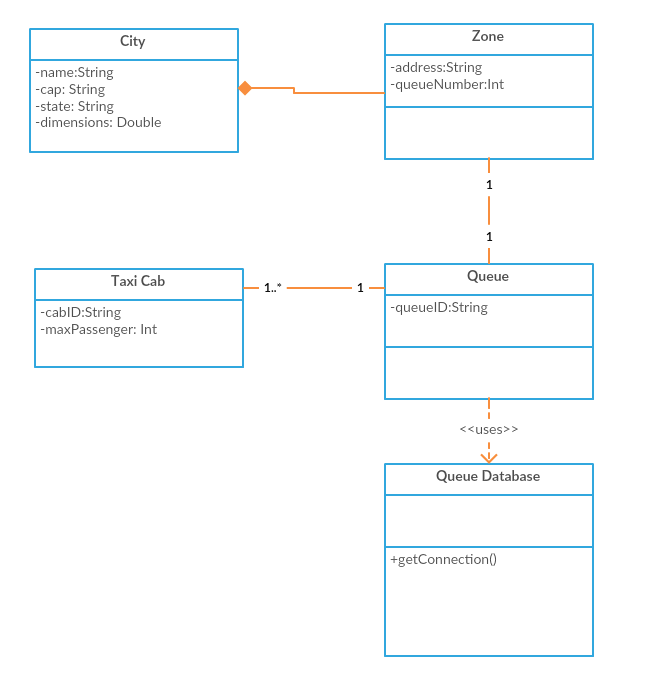
\includegraphics[scale=0.6]{req4}
\end{figure}
\clearpage
\item \textbf{Allow the client to reserve taxi for an exact time:}
\begin{itemize}
\item The system has to provide a functionality that allow the passenger to reserve a taxi for a desired time.
\end{itemize}
\vspace{3cm}
\begin{figure}[h]
\center 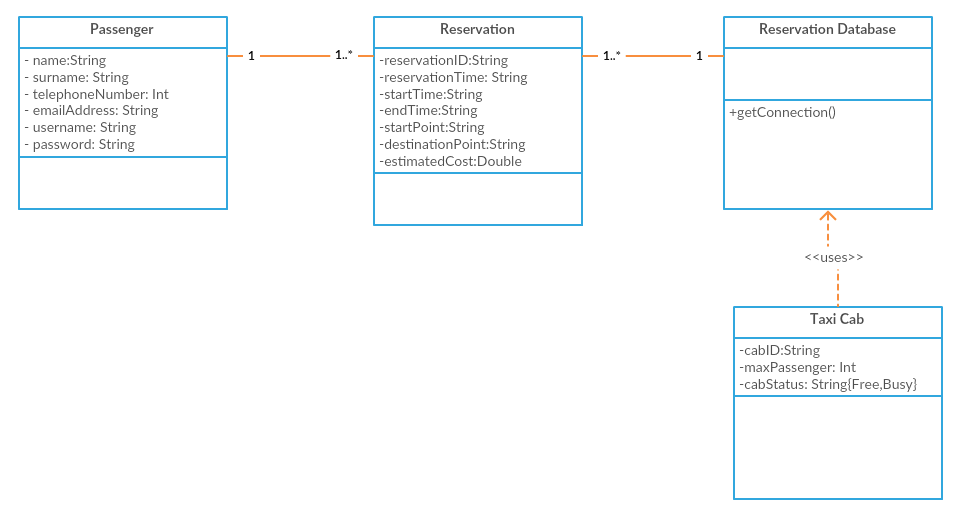
\includegraphics[scale=0.4]{req5}
\end{figure}
\end{enumerate}
\chapter{References}
\section{Software and used Tools}
\begin{itemize}
\item TexShop (http://pages.uoregon.edu/koch/texshop/), to redact this document
\item CreatelyApp (https://creately.com/app/), to create the class diagrams
\item Balsamiq Mockups (https://balsamiq.com/products/mockups/), to create the user interface mockup
\item Edraw Max(https://www.edrawsoft.com), to create the sequence diagrams
\item Microsoft Visio (https://products.office.com/it-it/visio/flowchart-software), to create the algorithmic part
\end{itemize}
\section{Working hours}
\textbf{Dimitar Anastasovski:} $\thicksim$30 hours
\\
\\
\textbf{Marco Colombo:} $\thicksim$30 hours
\section{Changelog}
Minor changes in the document
\end{document}  